%%%%%%%%%%%%%%%%%%%%%%%%%%%%%%%%%%%%%%%%%
% University/School Laboratory Report
% LaTeX Template
% Version 3.0 (4/2/13)
%
% This template has been downloaded from:
% http://www.LaTeXTemplates.com
%
% Original author:
% Linux and Unix Users Group at Virginia Tech Wiki 
% (https://vtluug.org/wiki/Example_LaTeX_chem_lab_report)
%
% License:
% CC BY-NC-SA 3.0 (http://creativecommons.org/licenses/by-nc-sa/3.0/)
%
%%%%%%%%%%%%%%%%%%%%%%%%%%%%%%%%%%%%%%%%%

%----------------------------------------------------------------------------------------
%	PACKAGES AND DOCUMENT CONFIGURATIONS
%----------------------------------------------------------------------------------------

\documentclass{article}

%\usepackage{mhchem} % Package for chemical equation typesetting
%\usepackage{siunitx} % Provides the \SI{}{} command for typesetting SI units

\usepackage{graphicx} % Required for the inclusion of images
\usepackage[top=1in,bottom=1in,right=1in,left=1in]{geometry}% Set the margins

%Multiple column picture packages
\usepackage{caption}
\usepackage{subcaption}

%Add code formating
\usepackage{listings}
\lstset{tabsize=2}

%Add support for floating images
\usepackage{float}

%Define the style for VHDL
\lstdefinelanguage{VHDL}{
  morekeywords={
    library,use,all,entity,is,port,in,out,end,architecture,of,
    begin,and
  },
  morecomment=[l]--
}

%Give the VHDL code color
\usepackage{xcolor}
\colorlet{keyword}{blue!100!black!80}
\colorlet{comment}{green!90!black!90}
\lstdefinestyle{vhdl}{
  language     = VHDL,
  basicstyle   = \ttfamily,
  keywordstyle = \color{keyword}\bfseries,
  commentstyle = \color{comment}
}

\usepackage{amssymb}
\usepackage{amsmath}

%Highlight command
\usepackage{tikz}
\usepackage{xspace}
\usetikzlibrary{decorations.pathmorphing}
\newcommand\hl[1]{%
    \tikz[baseline,%
      decoration={random steps,amplitude=1pt,segment length=15pt},%
      outer sep=-15pt, inner sep = 0pt%
    ]%
   \node[decorate,rectangle,fill=yellow,anchor=text]{#1\xspace};%
}%

% Create the header and footer
\usepackage{fancyhdr}
\pagestyle{fancy}
\lhead{CprE 583}
\rhead{Blake Vermeer, Kris Hall, Rohit Zambre}
\renewcommand{\footrulewidth}{0.4pt}

\setlength\parindent{0pt} % Removes all indentation from paragraphs

\renewcommand{\labelenumi}{\alph{enumi}.} % Make numbering in the enumerate environment by letter rather than number (e.g. section 6)

%\usepackage{times} % Uncomment to use the Times New Roman font

%----------------------------------------------------------------------------------------
%	DOCUMENT INFORMATION
%----------------------------------------------------------------------------------------

\title{MP-3 Write-Up} % Add title here...

\author{Blake \textsc{Vermeer}\\
		Kris \textsc{Hall}\\
		Rohit \textsc{Zambre}} % Author name

\date{\today} % Date for the report

\begin{document}

\maketitle % Insert the title, author and date

\begin{center}
\begin{tabular}{l r}
Date Due: & October 31, 2014 \\ % Date the assignment is due
%Partners: & James Smith \\ % Partner names (optional)
Instructors: & Joseph Zambreno % Instructor/supervisor
\end{tabular}
\end{center}

% If you wish to include an abstract, uncomment the lines below
% \begin{abstract}
% Abstract text
% \end{abstract}


% If you need to include a figure, copy the lines below
%\begin{figure}[H]
%	\begin{center}
%		\includegraphics[scale=0.35]{ADD FILE LOCATION OF PICTURE FILE HERE}
%		\caption{ADD CAPTION HERE}
%	\end{center}
%\end{figure}


%If you need to include VHDL code, copy the lines below and fill in the VHDL code
%\begin{center}
%	\begin{lstlisting}[style=vhdl]
%		VHDL CODE GOES HERE.	
%	\end{lstlisting}
%\end{center}

%----------------------------------------------------------------------------------------
%	SECTION 1
%----------------------------------------------------------------------------------------


\section{Overview}
In this lab we learned about the LEON processor on how to create and integrate a co-process with the LEON processor.


% If you have more than one objective, uncomment the below:
%\begin{description}
%\item[First Objective] \hfill \\
%Objective 1 text
%\item[Second Objective] \hfill \\
%Objective 2 text
%\end{description}

%\subsection{Definitions}
%\label{definitions}
%\begin{description}
%\item[Stoichiometry]
%The relationship between the relative quantities of substances taking part in a reaction or forming a compound, typically a ratio of whole integers.
%\item[Atomic mass]
%The mass of an atom of a chemical element expressed in atomic mass units. It is approximately equivalent to the number of protons and neutrons in the atom (the mass number) or to the average number allowing for the relative abundances of different isotopes. 
%\end{description} 
 
%----------------------------------------------------------------------------------------
%	SECTION 2
%----------------------------------------------------------------------------------------
\section{Software Grayscale Conversion}
After getting acquainted with the build environment for the LEON processor, we dived into the \textit{frameloop.c} code to see how it works. First we started by examining the main function and dissecting how it works. The main function of \textit{frameloop.c} first sets up the environment by enabling the coprocessor, and configuring and enabling the SVGA controller. It primarily copies all (= NFRAMES) of the image frames from memory to the SVGA controller; it can do so via two modes: mode 1 and mode 2. After the completion of the transfer of all (= NFRAMES) image frames, it computes the Frame Per Second measure for the buffering process. \\

Next we looked at the two different modes that were present in \textit{frameloop.c} to determine what they did. Mode 1 merely copies the current image from memory to the controller without applying any filters. Mode 2 is much more involved than mode 1. In mode 2, a filter is applied to each frame being transferred from memory to the buffer in the controller. Currently, two RGB values are being computed for each image frame and an OR is performed between the two RGB values to obtain the final the image frame that will be sent to the controller.

	 \begin{figure}[H]
	 	\begin{center}
	 		\includegraphics[scale=0.6]{../part4_files/Floating_Point_Grayscale_Screenshot.png}
	 		\caption{Floating Point Software Grayscale Conversion Results}
	 	\end{center}
	 \end{figure}
	 
	 \begin{figure}[H]
	 	\begin{center}
	 		\includegraphics[scale=0.6]{../part4_files/Fixed_point_grayscale_resluts_screenshot.png}
	 		\caption{Fixed Point Software Grayscale Conversion Results}
	 	\end{center}
	 \end{figure}


%----------------------------------------------------------------------------------------
%	SECTION 3
%----------------------------------------------------------------------------------------
\section{Hardware Coprocessor - Grayscale Conversion}
In this section we were asked to read through the code in \textit{coproc.vhd} and \textit{coproc\_core.vhd} and provide a description of how the controller sends data to the core. After reading over the code in \textit{coproc.vhd} it became apparent that the LEON processor was passing the entire program instruction to the coprocessor. From there the coprocessor parses the instruction and extracts the op-code and source and destination register addresses. After getting the source register addresses it pulls the data directly from these registers. Therefore, the coprocessor has direct access to the LEON processor's registers. \\

We based our hardware coprocessor for the grayscale conversion on the logic we used to implement the software grayscale conversion. Here is a hardware diagram for the coprocessor we designed:

	 \begin{figure}[H]
	 	\begin{center}
	 		\includegraphics[scale=0.6]{../part5_files/Grayscale_coprocessor_dataflow.png}
	 		\caption{Hardware Grayscale Conversion Coprocessor Dataflow Diagram}
	 	\end{center}
	 \end{figure}

The structure for the hardware coprocessor ended up being fairly simple and easily parallelized. Because of these qualities we were able to make the coprocesser complete the operation in one clock cycle. Additionally, since we were able to output a 64-bit value from the coprocessor, we are able to process four individual pixels in that single clock cycle. Including the load and storing operations (for some reason we could only get the 32-bit load/store operations to work correctly) it would only take 5 clock cycles (assuming the load and store operations take one cycle each).

%----------------------------------------------------------------------------------------
%   SECTION 4
%----------------------------------------------------------------------------------------
\section{Hardware Coprocessor - Edge Detection}
In this section, the task given is to modify the coprocessor to be able to perform greyscale edge detection. In order to implement this ability correctly, some changes had to be made to the files \textit{coproc.h}, \textit{coproc.vhd}, and \textit{coproc\_core.vhd}. The changes to the files were to provide two new instructions, CP\_PRELOAD, and CP\_EDGE\_DETECT.\\
In order to increase throughput, and potentially accelerate the process, the conclusion was made that the best approach to performing edge detection is as follows. Since the laplacian edge detection operation performed on a pixel requires the values of the eight pixels that surround it, a design decision made was that edge detection will not be performed on the pixels on the edge of the screen. 

	 \begin{figure}[H]
	 	\begin{center}
	 		\includegraphics[scale=0.6]{../part5_files/Fixed_point_greyscale_coprocessor_results.png}
	 		\caption{Fixed Point Coprocessor Grayscale Conversion Results}
	 	\end{center}
	 \end{figure}


%----------------------------------------------------------------------------------------
%	SECTION 4
%----------------------------------------------------------------------------------------
\section{Software Edge Detection}

	 \begin{figure}[H]
	 	\begin{center}
	 		\includegraphics[scale=0.6]{../part6_files/Software_Laplace_edge_software_performance.png}
	 		\caption{Software Laplace Edge Detection Results}
	 	\end{center}
	 \end{figure}


%----------------------------------------------------------------------------------------
%	SECTION 5
%----------------------------------------------------------------------------------------
\section{Hardware Coprocessor - Edge Detection}

	 \begin{figure}[H]
	 	\begin{center}
	 		\includegraphics[scale=0.6]{../part7_files/Hardware_Laplace_edge_detection_performance.png}
	 		\caption{Hardware Laplace Edge Detection Results}
	 	\end{center}
	 \end{figure}



%----------------------------------------------------------------------------------------
%	SECTION 6
%----------------------------------------------------------------------------------------
\section{Conclusion}



%----------------------------------------------------------------------------------------
%	BIBLIOGRAPHY
%----------------------------------------------------------------------------------------
%\newpage

%\bibliographystyle{unsrt}

%\bibliography{sample}

%----------------------------------------------------------------------------------------


\end{document}
